\documentclass{article}

\usepackage{minted}
\usepackage[most]{tcolorbox}
\usepackage{geometry}
\usepackage{enumitem}
\usepackage{hyperref}
\usepackage{hyperref}
\usepackage[parfill]{parskip}
\usepackage{wrapfig}
\usepackage{accsupp}

\geometry{margin=0.8in}
\definecolor{lightgreen}{rgb}{0.56, 0.93, 0.56}
\definecolor{moonstoneblue}{rgb}{0.45, 0.66, 0.76}
\definecolor{magenta}{rgb}{0.8,0.66,0.76}
\begin{document}
\begin{flushright}
Computational Biology ~\\
Tufts University Bio 35 ~\\
Fall 2021 ~\\ ~\\
\end{flushright}
\begin{center}{\textbf{\Large{Spotlight 12: Emilia Huerta-Sanchez}}}\end{center}

\textit{Please note that in general I have taken/adapted the words of our Spotlight subjects from their own websites to describe their work. I have done this in an effort to maintain accuracy in describing their research programs. Please do not copy paste text from their papers/websites in your assignments!}

\begin{wrapfigure}{L}{0.14\textwidth}
\begin{center}
 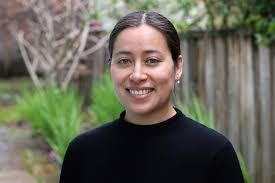
\includegraphics[width=0.13\textwidth]{images/huerta-sanchez.jpeg}
 \end{center}
\end{wrapfigure}
~\\ As part of our unit on human evolution, we will explore the work of Emilia Huerta-Sanchez. Prof. Huerta-Sanchez is a population geneticist interested in integrating theoretical, computational, and statistical modeling to address questions in human evolutionary biology. Her current research interests involve scanning human genomes from different populations to detect mutations in genes that have helped humans adapt to different environments like different diets, temperatures, pathogens and altitudes. She is a faculty member at Brown University.
~\\ ~\\

Please read the following article by Prof. Huerta-Sanchez: 
\begin{enumerate}
\item \texttt{\href{https://www.sciencedirect.com/science/article/pii/S0092867418312315}{https://www.sciencedirect.com/science/article/pii/S0092867418312315}}
\end{enumerate}

And the following news story about Prof. Huerta-Sanchez' work:
\begin{enumerate}
\item \texttt{\href{https://slate.com/technology/2014/07/tibetans-inherited-denisovan-genetic-adaptation-for-elevation-dna-for-living-at-high-altitude.html}{https://slate.com/technology/2014/07/tibetans-inherited-denisovan-...}}
\end{enumerate}

\subsubsection*{Written Assignment} 
After reading about Prof. Huerta-Sanchez' work, write a reflection (max one page) on what you discovered. You might wish to address some of the following: 

\begin{enumerate}
\item What was most interesting to you in reviewing these resources?
\item What did you learn from these resources about human evolution?
\item What new questions do you have after reviewing these resources?
\item What do these resources tell you about the types of people that do computational biology research, or their motivations?
\end{enumerate}

\EndAccSupp{}
\end{document}